Linking items and in general finding similarity among these already area-specific texts proved to be a problematic task. 

\subsection{NLTK}
\paragraph{Stack Overflow:}
The average similarity between SO questions talking about particular issue and that particular issue body description is 0.316 without body preprocessing and 0.292 with body preprocessing.

The distribution of similarities in buckets by increased by 0.05 can be seen in histogram in Figure 

\begin{figure}[H]%
    \centering
	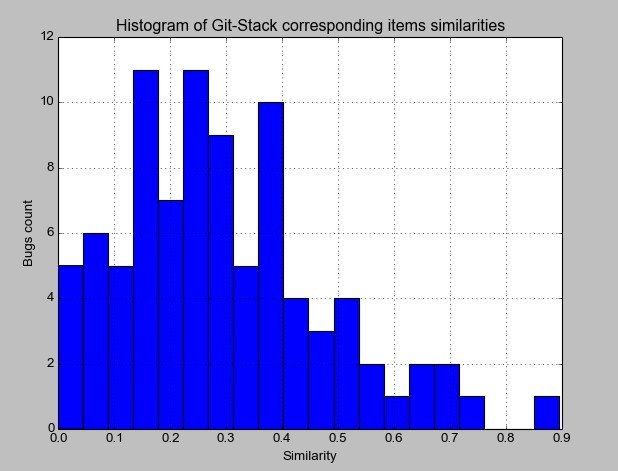
\includegraphics[width=8cm]{gitStackMatchesHistogram.jpg}
    \caption{Histogram of similarities distribution among git issues and their matching SO questions}%
    \label{fig:GitStackMatchesHistogram}%
\end{figure}



Comparing Git bugs descriptions with SO questions talking about own project issues and general issues, similarity values are following \ref{table:StackOverflowNLTKsimilarity}. Same table but for Reddit discussions can be seen in \ref{table:RedditNLTKsimilarity}

\begin{table}[H]
\centering
\begin{tabular}{ |p{3cm}||p{5cm}|p{5cm}|}
 \hline
\textbf{ Framework }& \textbf{Own issues similarity}& \textbf{All issues similarity}\\
 \hline
 NodeJS   & 0.265 & X\\ \hline
 Angular & 0.241 & X\\ \hline
 EmberJS & 0.282 & X\\ \hline 
 VueJS &   X & X\\ \hline
\end{tabular}
\caption{NLTK similarity values for SO questions}
\label{table:StackOverflowNLTKsimilarity}
\end{table}

\paragraph{Reddit:}
Here I've calculated the similarity between the bug description and either particular comment in the reddit discussion which mentioned the bug or the whole discussion itself. Average similarity score for all considered projects (NodeJS, AngularJS, VueJS and EmberJS) was 0.481 for the whole discussion and 0.396 for the comment itself. Detailed scores for each project can be found in table \ref{table:RedditNLTKsimilarity}. Subreddit for EmberJS didn't reference any of its own bugs.

\begin{table}[H]
\centering
\begin{tabular}{ |p{3cm}||p{3cm}|p{4cm}|}
 \hline
\textbf{ Framework }& \textbf{Bug comment}& \textbf{Whole discussion}\\
 \hline
 NodeJS   & 0.447 & 0.507\\ \hline 
 AngularJS & 0.306 & 0.57 \\ \hline 
 EmberJS & X & X\\ \hline
 VueJS &   0.359 & 0.380\\ \hline
\end{tabular}
\caption{Reddit NLTK similarity values}
\label{table:RedditNLTKsimilarity}
\end{table}

This indicates that the semantic meaning of the bug is better expressed in the whole discussion rather than just the particular comment which referenced the bug. This made me question if it could be generalized that longer the text is, more similar it is to actual bug description. I've plotted a relationship between similarity score and length in Figures \ref{fig:SimilarityLengthRelationshipComment} and \ref{fig:SimilarityLengthRelationshipDiscussion}.

\begin{figure}[H]%
    \centering
	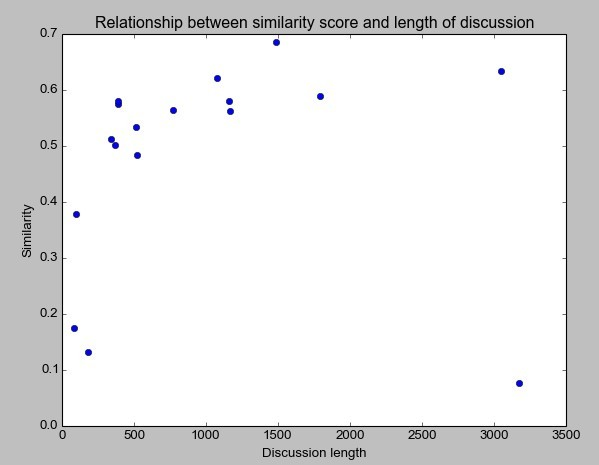
\includegraphics[width=8cm]{SimilarityLengthRelationshipDiscussion.jpg}
    \caption{Discussion lengths and similarity scores with the issue}%
    \label{fig:SimilarityLengthRelationshipDiscussion}%
\end{figure}

\begin{figure}[H]%
    \centering
	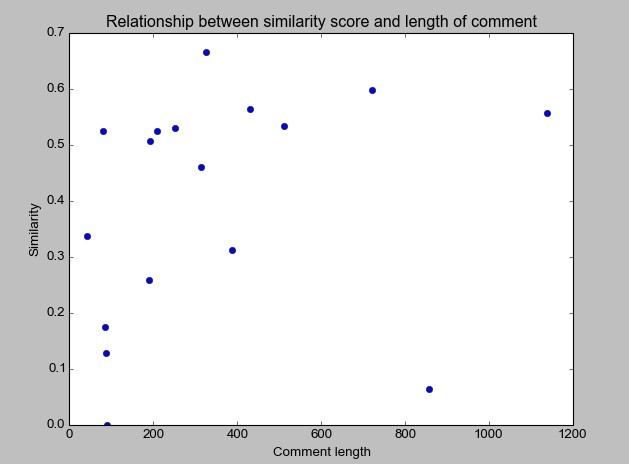
\includegraphics[width=8cm]{SimilarityLengthRelationshipComment.jpg}
    \caption{Comment lengths and similarity scores with the issue}%
    \label{fig:SimilarityLengthRelationshipComment}%
\end{figure}


